\documentclass[12pt,a4paper,utf8]{ctexart}
\usepackage{ctex,amsmath,amssymb,subfig,cite,graphicx,diagbox,fontspec,fancyhdr,geometry}
\usepackage[ntheorem]{empheq}
\usepackage{enumitem,fullpage,cleveref,cellspace,listings,color,framed}
\definecolor{gray}{rgb}{0.5,0.5,0.5}
\definecolor{dkgreen}{rgb}{.068,.578,.068}
\definecolor{dkpurple}{rgb}{.320,.064,.680}

%set Fortran styles
\lstset{
    frameround=tftf,
    language=Fortran,
    keywords={SELECT,PROGRAM,PRINT,STOP,END,WRITE,INTEGER,REAL,COMPLEX,CHARACTER,LOGICAL,READ,FORMAT,IMPLICIT,PARAMETER,DATA,EQUIVALENCE,TYPE,PAUSE,CONTINUE,CYCLE,EXIT,IF,SELECT,DO,ALLOCATE,DEALLOCATE,WHERE,FORALL,SUBROUTIHNE,CALL,RETURN,FUNCTION,COMMON,BLOCK DATA,SAVE,INTERFACE,CONTAIN,MODULE,USE,PUBLIC,PRIVATE,ENTRY,OPEN,INQUIRE,CLOSE,NAMELIST,POINTER,NULLFY,REWIND,BACKSPACE,ENDFILE
    },
    basicstyle=\small\ttfamily,
    numbers=left,
    numberstyle=\small,
    keywordstyle=\color{blue}\bfseries,
    commentstyle=\color{dkgreen},
    stringstyle=\color{dkpurple},
    backgroundcolor=\color{white},
    tabsize=2,
    showspaces=false,
    showstringspaces=false,
    breaklines=true,
    frame=trBL,
}
\CTEXsetup[format+={\raggedright}]{section}
\setlength{\parindent}{2em}
\geometry{
    textwidth=138mm,
    textheight=215mm,
    left=27mm,
    right=27mm,
    top=25.4mm,
    bottom=25.4mm,
    headheight=2.17cm,
    headsep=4mm,
    footskip=12mm,
    heightrounded,
}
\pagestyle{fancy}
\lhead{\textsl{2021秋-计算物理A}}
\chead{}
\rhead{\textsl{PB19020634-于浩然}}
\lfoot{}
\cfoot{\thepage}
\rfoot{}

\begin{document}
\begin{center}
    {\LARGE\textbf{计算物理作业六}}\\
    \textrm{于浩然}~~~~~~\textrm{PB19020634}~~~~~~\textrm{2021.10.20}
\end{center}

\section{作业题目}

对两个函数线型(Gauss分布和类Lorentz型分布),设其一为
$p(x)$,另一为$F(x)$,其中常数 $a \neq b \neq 1$,用舍选法对
$p(x)$抽样.将计算得到的归一化频数分布直方图与理论曲线$p(x)$进行比较,讨论差异,讨论抽样效率。
\begin{equation}
    \textrm{Gaussian}: \sim \exp (-ax^2); \qquad \textrm{Lorentzian like}: \sim
    \frac{1}{1 + bx^4}
\end{equation}

\begin{figure}[htp]
    \centering
    \includegraphics[width=0.8\textwidth]{tit.png}
    \caption{Gauss分布和类Lorentz型分布示意图}
\end{figure}    
\section{算法简介}
\subsection{Gauss分布/正态分布}

若随机变量 $X$服从位置参数为$\mu$、尺度参数为$\sigma$的正态分布,记为$X \sim
N(\mu, \sigma^2)$,则其概率密度函数为
\begin{equation}
    f(x) = \frac{1}{\sigma \sqrt{2\pi}} e^{- \frac{(x - \mu)^2}{2 \sigma ^2}}
\end{equation}

题干(1)所给Gaussian分布$f(x) = \exp (-ax^2)$,即平均值
$\mu=0$,$\sigma = 1/ \sqrt{2a}$,忽略了前面的归一化常系数.

\subsection{类Lorentz分布}

有一种物理学中十分重要的分布称为柯西-洛伦兹分布,它是描述受迫共振的微分方程的解:
\begin{equation}
    f(x;x_0,\gamma) = \frac{1}{\pi} \left[ \frac{\gamma}{(x-x_0)^2 + \gamma^2}
    \right]
\end{equation}

$x_0 = 0$且 $\gamma = 1$的特例称为柯西分布,概率密度函数为:
\begin{equation}
    f(x;0,1) = \frac{1}{\pi(1+x^2)}
\end{equation}

题目中所给“类Lorentz分布”便为将上式中$x^2$替换为$x^4$,稍微复杂一些.

具体到图1中的各条曲线,推测
\color{red}{红色为Gaussian分布} \color{black},\color{blue}{另两条可能是}
\color{green}{类Lorentz分布}\color{black}.

\subsection{舍选抽样法}

首先我们将作为概率密度函数的$p(x)$归一化,得到:
\begin{equation}
    p(x) = \sqrt{ \frac{a}{\pi}}e^{-ax^2}
\end{equation}

在本题中,$F(x)$并没有概率密度函数的物理含义,而仅仅作为舍选法中的比较函数,故不需要归一化.只需恰当选取$b$的值,使得在某一确定范围内$F(x)
\geq p(x)$,满足作为比较函数的要求.不妨设
\begin{equation}
    F(x) = \frac{k}{1+bx^4},\qquad k = const.
\end{equation}

按照舍选法的一般步骤:
\begin{enumerate}
    \item[(1)] 产生一对$[0,1]$区间中均匀分布的随机抽样值$(\xi_1 ,
        \xi_2)$,并求出抽样表示式:
        \begin{equation}
            \xi_1 = \frac{\int _{-\infty} ^{\xi_x} F(x) \textrm{d}x }{\int
            _{-\infty} ^{\infty} F(x) \textrm{d}x},\qquad \xi_y = \xi_2 F(\xi_x)
        \end{equation}

    \item[(2)] 判断如下条件是否成立:
        \begin{equation}
            \xi_y \leq p(\xi_x)
        \end{equation}
        若否,则舍,再次抽样;若是,则取$x = \xi
        _x$作为抽样结果.上面式中$F(x)$的积分形式复杂,难以用$\xi_1$解析表示出$\xi_x$,考虑逐次求数值解,在下一部分中我们将进一步讨论.
\end{enumerate}

\subsection{抽样变换式的进一步讨论}

$p(x)$和$F(x)$式中,$x$均取遍$(-\infty,
\infty)$.但在我们的实际抽样中只能考虑有限区间的抽样;而且结合了分布函数的特点(类似正态分布的$3\sigma$原则),我们知道距离中心点一定距离以外概率密度函数已经变得相当小,即使包含了这些区域抽样也未必能抽到这些点,如图2展示.

\begin{figure}[h]
    \centering
    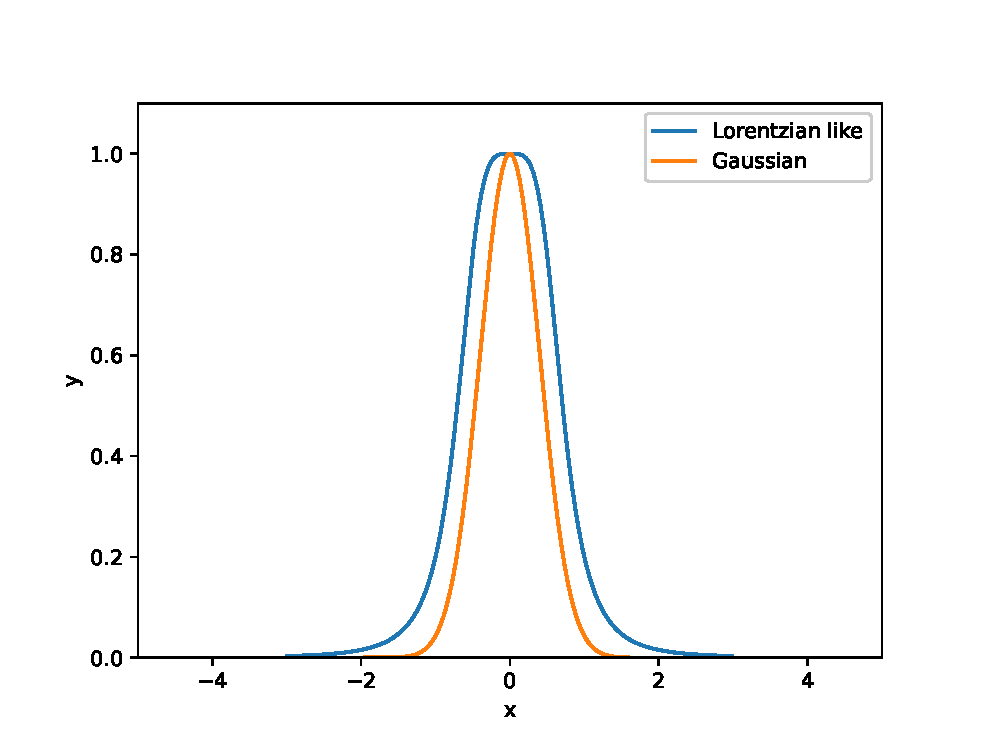
\includegraphics[width=0.8\textwidth]{funcfig.eps}
    \caption{两种函数线型示意图,取归一化的$a= \pi$,$F(x)= \frac{1}{1+4x^4}$}
\end{figure}

可以非常明显地看出,当$|x| > 3$时两曲线都明显趋近于零.于是有
\begin{equation}
    \int _{-3} ^3 F(x) \textrm{d}x \approxeq \int _{-\infty } ^{\infty} F(x)
    \textrm{d}x,\quad
    \int _{-3} ^3 p(x) \textrm{d}x \approxeq \int _{-\infty } ^{\infty} p(x)
    \textrm{d}x,\quad 
\end{equation}

为了后续编写程序,我们不妨设
\begin{equation}
    p(x) = e^{-\pi x^2}, \qquad F(x) = \frac{1}{1+4x^4}
\end{equation}

用Wolfram Alpha计算不定积分:
\begin{equation}
    \int \frac{ \textrm{d}x}{1+4x^4} = \frac{1}{8} \log{ \frac{2x^2+2x+1}{2x^2-2x+1}} -
    \frac{1}{4} \arctan (1-2x)+ \frac{1}{4}\arctan (2x+1) \equiv g(x)
\end{equation}

则
\begin{equation}
    \int _{-\infty} ^{\infty} F(x) \textrm{d}x \approxeq \int _{-3} ^{3} F(x)
    \textrm{d}x \approx 1.56463163641954 \equiv S		
\end{equation}
\begin{eqnarray}
    \int _{-\infty} ^{\xi_x} F(x) \textrm{d}x &\approxeq& \int _{-3} ^{\xi_x} F(x)
    \textrm{d}x \nonumber \\
                                              &=&
                                              g(\xi_x) - g(-3)
\end{eqnarray}

由(7)式,
\begin{equation}    
    S \xi_1 = g(\xi_x) -g(-3)
\end{equation}


对于每个给定$\xi_1$,可由上面方程解出$\xi_x$数值解,我们考虑使用 \textbf{弦截法}.

\subsection{弦截法求方程数值解}

弦截法是求非线性方程近似根的一种线性近似方法,是牛顿迭代法的一种变形算法.
对于非线性方程:
\begin{equation}
    f(x) = 0
\end{equation}
其迭代公式为:

\begin{equation}
    x_{k + 1} = x_k - \frac{(x_k - x_{k-1})f(x_k)}{f(x_k) - f(x_{k-1})}
\end{equation}

计算步骤为:
\begin{enumerate}
    \item[(1)] 选择迭代初值$x_0$、$x_1$以及误差精度$\varepsilon$

    \item[(2)] 按照迭代公式(15)计算$x_2$

    \item[(3)] 若 $|x_1 - x_0| < \varepsilon$,转向(4),否则$x_0 = x_1,x_1 =
        x_2$,返回(2)

    \item[(4)] 输出满足精度的根$x_2$,结束.

这种做法通过几次迭代就可以达到较好的精度,可以尝试在程序中使用.

\end{enumerate}
\section{编程实现}

很遗憾,数值计算过于复杂,也可能是前面的推导有误,程序不能输出正确的抽样结果.Anyway,还是
把程序代码贴在下面:

\begin{framed}
\begin{lstlisting}[language=Fortran]
MODULE Sam !抽样程序模块
    IMPLICIT NONE
    REAL(KIND=8) ,PARAMETER :: S = 1.56463163641954 !为了定义S这一全局变量使用模块
    REAL(KIND=8) ,PARAMETER :: PI = 3.1415926

    CONTAINS
    FUNCTION F(x)
        REAL(KIND=8) :: F, x
        F = 1 / (1 + 4 * x**4)
    END FUNCTION F
    FUNCTION P(x)
        REAL(KIND=8) :: P, x
        P = exp(-PI * x**2)
    END FUNCTION P
    FUNCTION G(x) !用函数定义g(x)表达式
        REAL(KIND=8) :: G, x
        G = log((2 * x**2 + 2 * x + 1)/(2 * x**2 - 2 * x + 1)) / 8 + atan(1 - 2 * x) / 4 + atan(1 + 2 * x) / 4
    END FUNCTION G
    FUNCTION H(x, xi_1) !定义要求解的方程左端h(x)
        REAL(KIND=8) :: xi_1, H, x
        H = G(x) - G(-3.0_8) - S * xi_1
    END FUNCTION H

    FUNCTION Sec(x0, x1, err, xi_1) !弦截法(Secant Method)求方程数值解
        REAL(KIND=8) ,INTENT(IN) :: err, x0, x1, xi_1
        REAL(KIND=8) :: Sec, tmp, tmpx0, tmpx1, diff
        INTEGER(KIND=8) :: i
        tmpx0 = x0
        tmpx1 = x1
        diff = x1 - x0
        DO WHILE (diff > err)
            tmp = tmpx1
            tmpx1 = tmpx1 - (tmpx1 - tmpx0) * H(tmpx1, xi_1) / (H(tmpx1, xi_1) - H(tmpx0, xi_1))
            tmpx0 = tmp
            diff = tmpx1 - tmpx0
        END DO
        Sec = tmpx1
    END FUNCTION Sec

    SUBROUTINE Sample(n) !进行舍选法抽样
        REAL(KIND=8) ,DIMENSION(10**n) :: x, y, xi_x, xi_y
        INTEGER(KIND=4) :: n, i
        REAL(KIND=8), DIMENSION(10**n) :: z !数组用于存放抽样结果
        OPEN (1, file='x.dat')
        READ (1, *) x
        CLOSE (1)
        OPEN (1, file='y.dat')
        READ (1, *) y
        CLOSE (1)
        DO i = 1, 10**n
            xi_x(i) = Sec(-3.0_8, 3.0_8, 0.00001_8, x(i)) !全部按照种别值为8传入参数
            print *, xi_x(i)
            IF (y(i) * F(xi_x(i)) < P(xi_x(i))) THEN
                z(i) = xi_x(i)
            END IF
        END DO
    END SUBROUTINE Sample
END MODULE Sam

SUBROUTINE Schrage(P, z0, filename) !Schrage随机数生成器子程序
    IMPLICIT NONE
    INTEGER :: N = 1, P
    INTEGER :: m = 2147483647, a = 16807, q = 127773, r = 2836, In(10**P), z0
    REAL(KIND=8) :: z(10**P)
    CHARACTER(LEN=5) :: filename
    In(1) = z0 !将传入值z0作为种子
    z(1) = REAL(In(1))/m
    DO N = 1, 10**P - 1
        In(N + 1) = a*MOD(In(N), q) - r*INT(In(N)/q)
        IF (In(N + 1) < 0) THEN !若值小于零,按Schrage方法加m
            In(N + 1) = In(N + 1) + m
        END IF
        z(N + 1) = REAL(In(N + 1))/m !得到第N+1个随机数
    END DO
    OPEN (1, file=filename) !每次运行子程序按照传入参数filename生成数据文件
    DO N = 1, 10**P !将随机数按行存入文件
        WRITE (1, *) z(N)
        END DO
    CLOSE (1)
END SUBROUTINE Schrage

PROGRAM MAIN

    USE Sam
    INTEGER(KIND=4) :: intI = 4
    CALL Schrage(intI, 84651212, 'x.dat') !产生一对[0,1]之间均匀分布的随机数
    CALL Schrage(intI, 16545214, 'y.dat')
    CALL Sample(intI)
END PROGRAM MAIN
\end{lstlisting}
\end{framed}
\section{结论}

本题中虽然未求出抽样结果,但由于要使用全局常量的缘故了解了FORTRAN90中函数、模块的结构与使用
,有助于后面其他程序的设计.对于如同本题中$F(x)$这样比较复杂的函数难以求解积分,故以其作为比较函数会造成极大的麻烦.
当使用舍选抽样法时,还应选择形式尽量简单的比较函数.
\end{document}
